% Generated from the public primitive catalog. Original Atlas drawing; Apache-2.0.
% Target: keccak; view: overview-compact
\documentclass[border=9pt]{standalone}
% Original Atlas figure theme. Apache-2.0; see the repository LICENSE.
\usepackage[T1]{fontenc}
\usepackage{lmodern}
\usepackage{amsmath,amssymb}
\usepackage{tikz}
\usetikzlibrary{arrows.meta,positioning,calc,fit,backgrounds,decorations.pathreplacing,matrix}
\definecolor{atlasInk}{HTML}{172235}
\definecolor{atlasTeal}{HTML}{0D7B7D}
\definecolor{atlasMuted}{HTML}{637278}
\definecolor{atlasFill}{HTML}{EAF4F2}
\definecolor{atlasLine}{HTML}{B6C8C7}
\tikzset{
  every picture/.style={line width=.65pt,draw=atlasInk,>=Latex},
  every node/.style={text=atlasInk,font=\sffamily\small},
  box/.style={draw,rounded corners=1.5pt,minimum height=.9cm,minimum width=1.6cm,align=center,inner sep=6pt,fill=white},
  accent/.style={box,draw=atlasTeal,fill=atlasFill},
  wire/.style={->,line width=.7pt},
  keywire/.style={wire,draw=atlasTeal,dashed},
  xor/.style={draw,circle,fill=white,inner sep=0pt,minimum size=.38cm},
  add/.style={draw,rectangle,fill=white,inner sep=0pt,minimum size=.38cm},
  note/.style={font=\sffamily\scriptsize,text=atlasMuted,align=center},
  phase/.style={font=\sffamily\small\bfseries,text=atlasTeal},
  group/.style={draw=atlasLine,dashed,rounded corners=2pt,inner sep=8pt}
}
\newcommand{\rotl}{\mathbin{\lll}}
\newcommand{\rotr}{\mathbin{\ggg}}
\newcommand{\kx}{\operatorname{Keccak}\!\text{-}\!f[1600]}

\newcommand{\AtlasKeyBits}{k}
\newcommand{\AtlasKeyWords}{N_k}
\newcommand{\AtlasRounds}{n}
\newcommand{\AtlasPriorRounds}{N_r-1}
\newcommand{\AtlasRoundKeys}{N_r+1}
\newcommand{\AtlasDoubleRounds}{N_r/2}
\newcommand{\AtlasSixRoundGroups}{N_r/6}
\newcommand{\AtlasFLGroups}{N_r/6-1}
\newcommand{\AtlasRoundStart}{24-n}
\newcommand{\AtlasBlockBits}{b}
\newcommand{\AtlasOutputBits}{d}
\newcommand{\AtlasStateBits}{1600}
\newcommand{\AtlasNonceBits}{v}
\newcommand{\AtlasCounterBits}{q}
\newcommand{\AtlasStreamBlockBits}{b}
\newcommand{\AtlasRate}{r}
\newcommand{\AtlasCapacity}{c}
\newcommand{\AtlasSteps}{N}
\newcommand{\AtlasLastStep}{N-1}
\newcommand{\AtlasWordBits}{200}
\newcommand{\AtlasHashWords}{50}
\newcommand{\AtlasFeedForward}{\boxplus}
\newcommand{\AtlasByteOrder}{big-endian}
\newcommand{\AtlasDomain}{01}
\newif\ifAtlasXof
\AtlasXoffalse
\begin{document}
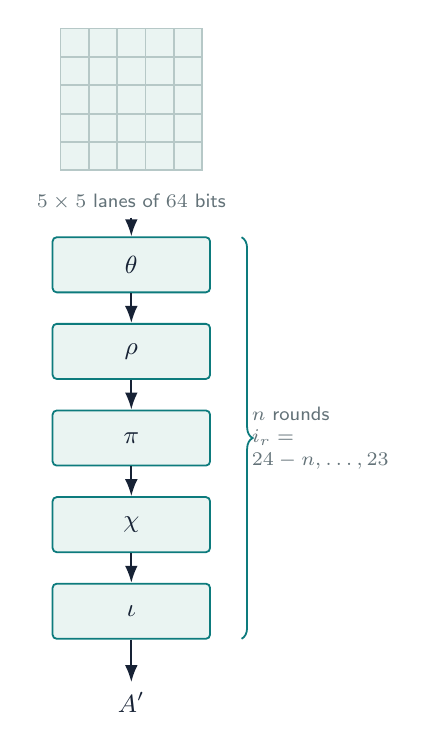
\begin{tikzpicture}
  \foreach \x in {0,...,4} \foreach \y in {0,...,4} {
    \draw[draw=atlasLine,fill=atlasFill] (-.9+.36*\x,1-.36*\y) rectangle ++(.36,-.36);
  }
  \node[note] at (0,-1.2) {$5\times5$ lanes of $64$ bits};
  \foreach \y/\name/\label in {-2/theta/\theta,-3.1/rho/\rho,-4.2/pi/\pi,-5.3/chi/\chi,-6.4/iota/\iota} {
    \node[accent,minimum width=2cm,minimum height=.7cm] (\name) at (0,\y) {$\label$};
  }
  \draw[wire] (0,-1.4) -- (theta); \draw[wire] (theta) -- (rho); \draw[wire] (rho) -- (pi);
  \draw[wire] (pi) -- (chi); \draw[wire] (chi) -- (iota);
  \draw[decorate,decoration={brace,amplitude=4pt},draw=atlasTeal] (1.4,-1.65) -- (1.4,-6.75);
  \node[note,align=left] at (2.4,-4.2) {$\AtlasRounds$ rounds\\$i_r=$\\$\AtlasRoundStart,\ldots,23$};
  \draw[wire] (iota) -- (0,-7.3) node[below] {$A'$};
\end{tikzpicture}

\end{document}
